The Proton Synchrotron (PS) is part of the injector chain and is used to accelerate particles from the Proton Synchrotron Booster (PSB) to the SPS and finally to the Large Hadron Collider (LHC). For the purpose of CHIMERA, it can also be receive and accelerate heavy ions from the Low Energy Ion Ring (LEIR) and extract them to the East Area. The PS uses radio frequency (RF) cavities to accelerate charged particles, such as protons or Pb ions, to high energies and uses 100 dipoles to bend the beam around its 628 m circumference \cite{}. These particles are then extracted using slow extraction through a beam line and transported to the CHARM facility, where the CHIMERA instruments are located.

The beam energy refers to the kinetic energy per nucleon $E_{kin}$ of the charged particle beam. The relationship for an ion beam is $E_{kin, TOT}=E_{kin}\cdot A$, where A is the atomic mass number (A = Z + N, the number of protons Z and neutrons N). The total momentum for an ion beam is \cite{chao_handbook_2013}

$$pc={E_{0}\sqrt{\gamma^{2}-1}}$$

$$pc = E_{0}\sqrt{\left [ \left( \frac{E_{kin}}{E_{0}}+1\right )^{2}-1\right ]}$$

where, $E_{0}$ is the rest mass of the ion and $\gamma=\frac{E}{E_{0}}=\frac{E_{0}+E_{cin}}{E_{0}} = \frac{E_{cin}}{E_{0}}+1$

The rigidity will be used to calculate the magnetic field used in the bending magnets of the PS and is defined as:
$$B\rho = \frac{pc}{q}$$

The CHIMERA beam uses a lead ion beam. During acceleration, the beam is a Pb54+ ion beam of partially stripped electrons (which means that it has 54 charges and 28 $e^{-}$ remaining) of isotope A=208. As an example for a 1 GeV per nucleon, the momentum would be:

$$pc = E_{0}\sqrt{\left [ \left( \frac{1\text{ [GeV]}\cdot 208}{E_{0}}+1\right )^{2}-1\right ]}$$

where the rest mass $E_{0}$ of Pb54+ is:

$$E_{0} = m_{Pb54+}= 82\cdot m_{proton} + 126\cdot m_{neutron} + 28\cdot m_{e^{-}} - m_{defect} = 193.74 \frac{\text{GeV}}{\text{c}^{2}}$$

with the mass defect: $m_{defect}=82\cdot m_{proton} + 126\cdot m_{neutron} + 28\cdot m_{e^{-}} - 208\cdot m_{u}$ 

\begin{table}[h!]
\centering
\begin{tabular}{lr}
\toprule
Particle & mass GeV/$\text{c}^{2}$\\
\midrule
$m_{proton}$ & 0.93828      \\
$m_{neutron}$ & 0.93957      \\
$m_{e^{-}}$ & 0.000511 \\
$m_{u}$ & 0.9315       \\
\bottomrule
\end{tabular}
\caption{Rest masses \cite{boston_university_nuclear_nodate}.}
\label{table:masses}
\end{table}

The conversion of beam momentum to rigidity in Tesla meter is done with: 
$$B\rho \text{ [T m]} = 3.3356\cdot p \text{ [GeV/c]}$$
where for the PS, $\rho = 70.0789$ m.

For the ESA run, three energies were selected: 1000, 750 and 650 MeV/nucleon. The associated magnetic field (B-field) required to which the ions will be accelerated to were calculated, see Fig. \ref{fig:lookup table} and Table \ref{table:KE_table}. Two different momentas are needed for acceleration and transport respectively as the ion beam is partially stripped in the PS and become fully stripped after the exit vaccum windows in the F61 transfer line located after the first quadrupole Q74L. The magnets in the transfer line must be pulsed with a rigidity associated to the newly fully stripped ion beam. Extensive work as been done to scale the magnets in F61 and the T8 transfer line. A makerule is used to calculate the correct strength to apply according to the PS B-field (and thus beam energy). The makerule calculate a partially stripped momenta for the first quadrupole in F61 and a second momenta for a fully stripped ion beam for the rest of the transfer line down to CHARM. This automatic scaling is extremely useful as energy scans can be done by simply changing the Bfield at flattop of the PS. Some limitations are that the extraction path and the SMH57 and SMH61 sometimes need small manual corrections and the bending to the East dump do not have a makerule associated yet (only current can be chosen).

\begin{figure}[!htb]
\centering
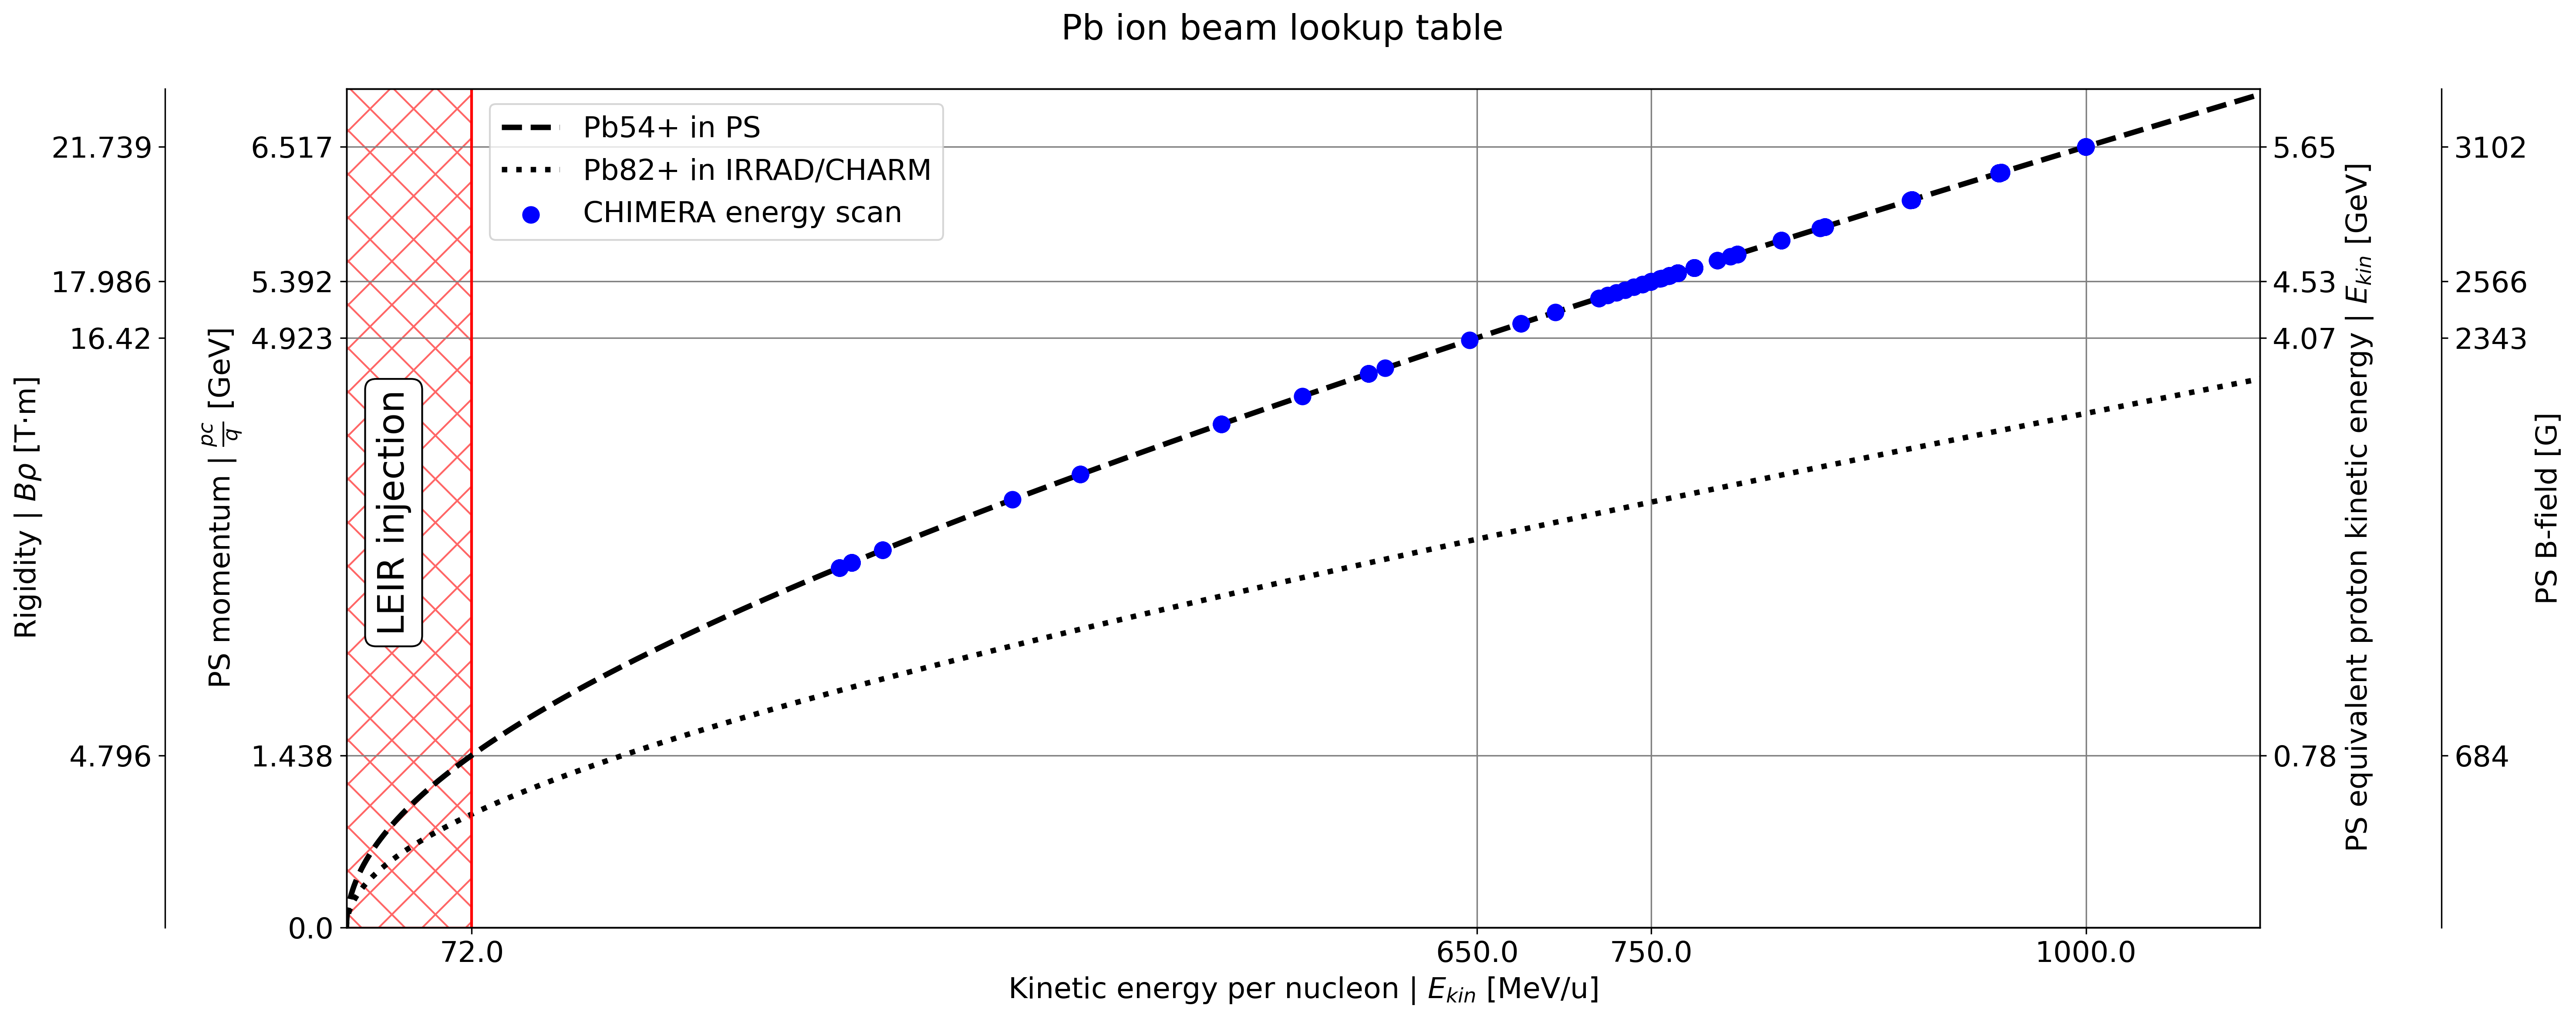
\includegraphics[width=1.0\textwidth]{images/kinetic_energy_lookup_chimera.png}
\caption{Lead ion beam lookup table. In addition, measurement to the East dump with an energy scan is shown.}
\label{fig:lookup table}
\end{figure}

Figure \ref{fig:bfield} shows the shape of the magnetic field in the main dipoles of the PS produced by the Power system for the PS main magnet (POPS). There are two main regions, the injection plateau and the flat-top extraction plateau. The spike at the end to circumvent some limitation of POPS should be disregarded, as the extraction is done prior to this event.

\begin{figure}[!htb]
\centering
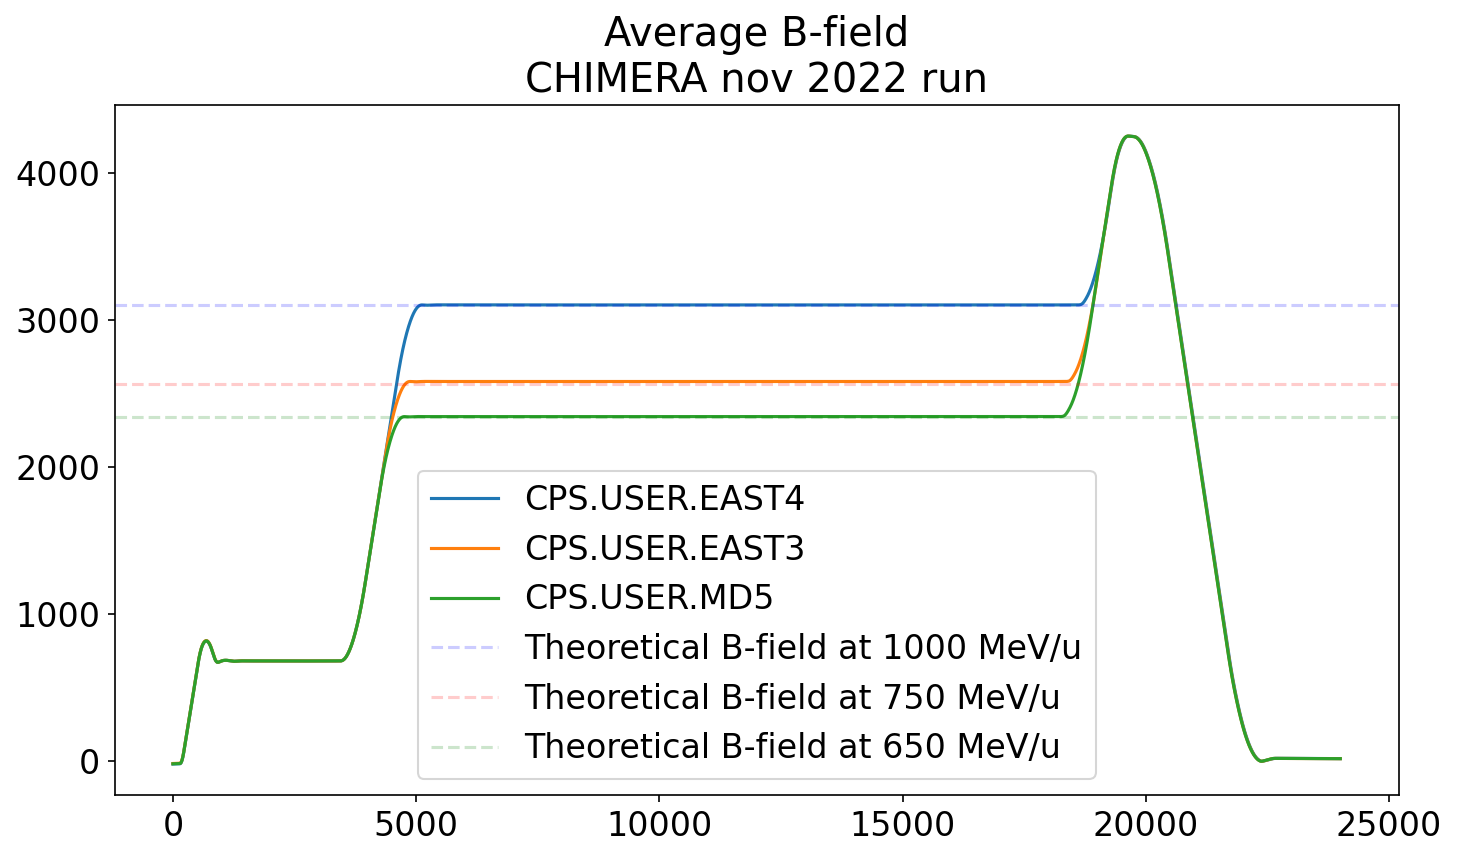
\includegraphics[width=0.8\textwidth]{images/average_b_field_chimera.png}
\caption{CHIMERA B-field for different energies. There are two plateaus: the injection plateau at 684 G and then extraction plateaus at different B-field corresponding to different energies.}
\label{fig:bfield}
\end{figure}

\begin{table}[h!]
\centering
\begin{tabular}{rrrrl}
\toprule
 $E_{kin}$ [MeV/nucleon] &  $\frac{pc}{54}$ [GeV] &  $\frac{pc}{82}$ [GeV] &  PS B-field [G] & User mapping\\
\midrule
  1000 &                        6.517 &                    4.292 &        3102 & CPS.USER.EAST4 \\
   750 &                        5.392 &                    3.551 &        2566 & CPS.USER.EAST3 \\
   650 &                        4.923 &                    3.242 &        2343 &   CPS.USER.MD4 \\
\bottomrule
\end{tabular}
\caption{Kinetic energy used during the ESA november 2022 run. The momentum/charge for a partially stripped and fully stripped ion beam is shown.}
\label{table:KE_table}
\end{table}

\begin{figure}[!htb]
\centering
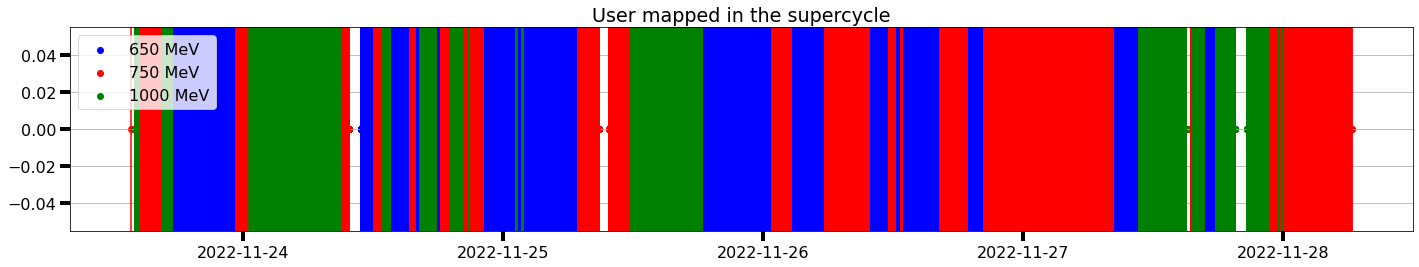
\includegraphics[width=1.0\textwidth]{images/Pasted image 20221130110611.png}
\caption{Timestamp of different energies}
\label{fig:timestamp_energies}
\end{figure}

For development purposes and after the ESA run, an automatic script was used to ramp the beam energy. The lowest beam energy seen on the East Dump was 283 MeV/nucleon and lower energies could be tried out in the future. The main limitation during this run was that the bending magnet to the dump is not scaled with momentum and hand corrections were needed to propagate the beam to the dump as well as the beam spot on the BTV at this energy was large and weak which made observation difficult.


\begin{figure}
    \centering
    \begin{minipage}{0.45\textwidth}
        \centering
        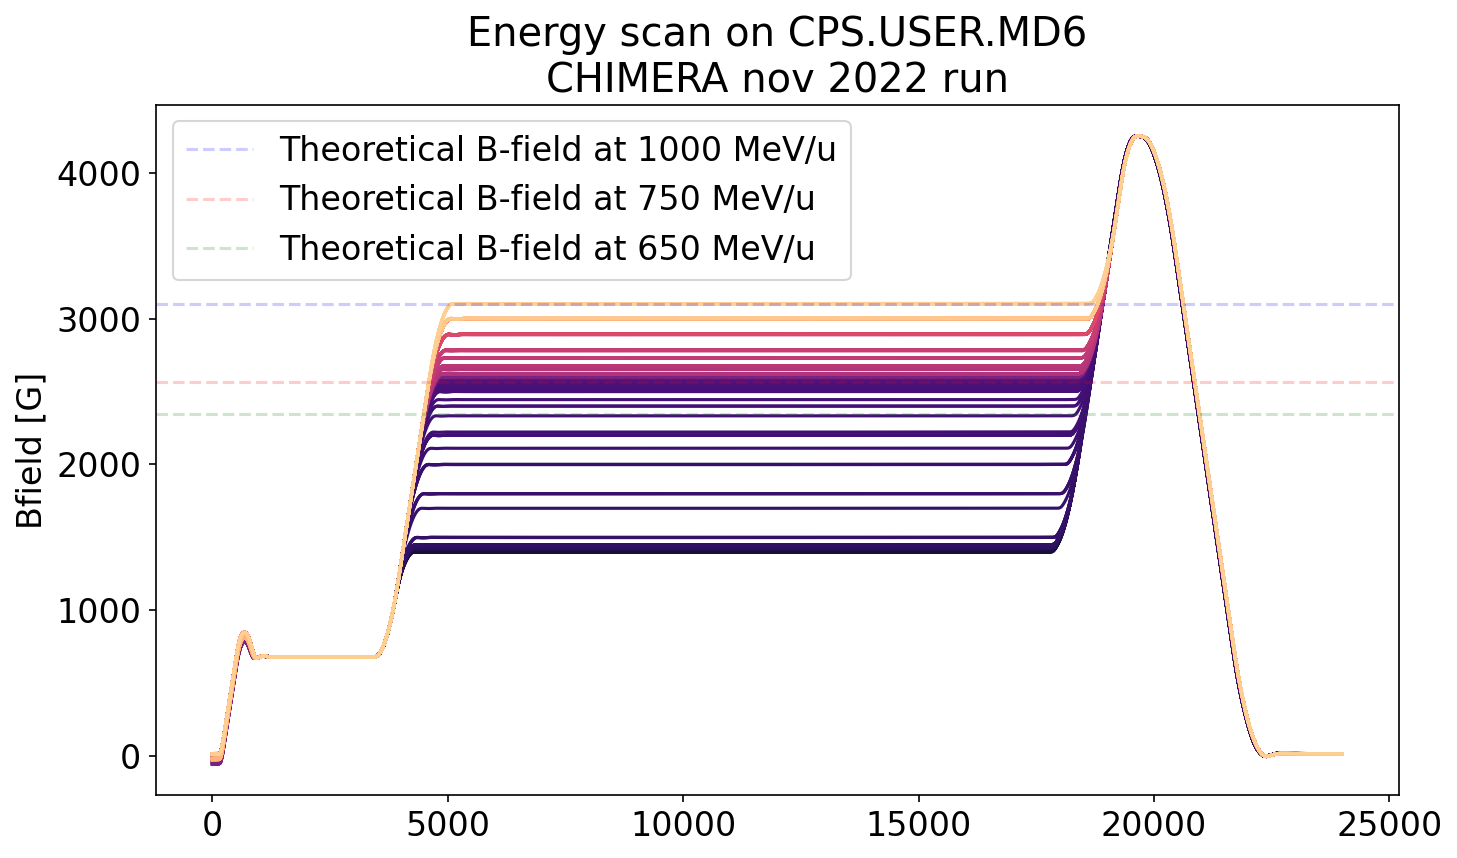
\includegraphics[width=1.0\textwidth]{images/energy_scan_chimera 1.png}
        \caption{Energy scan}
        \label{fig:energy_scan}
    \end{minipage}\hfill
    \begin{minipage}{0.45\textwidth}
        \centering
        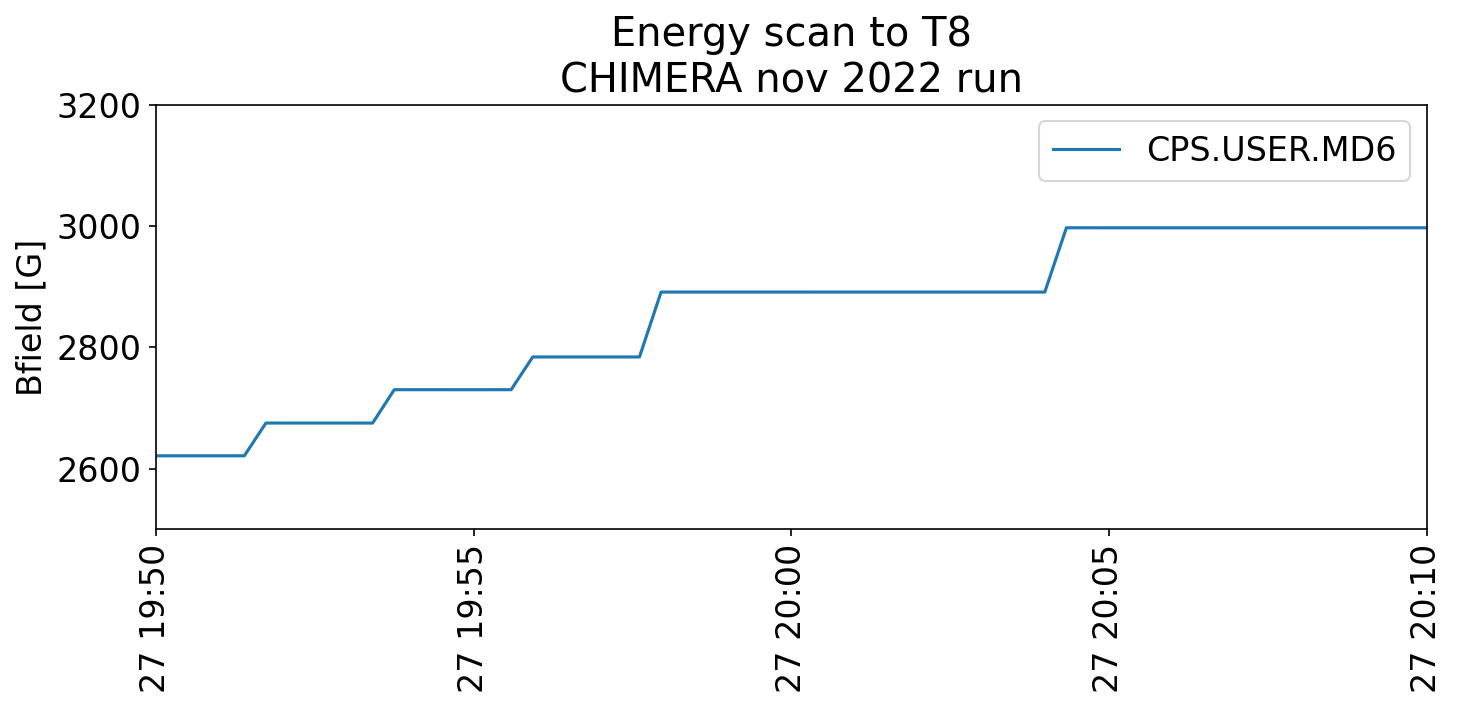
\includegraphics[width=1.0\textwidth]{images/energy_scan_timestamp_chimera 1.png} 
        \caption{Energy scan with timestamp}
        \label{fig:energy_scan_timestamp}
    \end{minipage}
\end{figure}

\subsection{Slow extraction}

The ion slow extraction scheme uses the magnetic septums SMH57 and SMH61 to extract the beam to the east area. As opposed to a proton slow extraction, for CHIMERA we bypasses the electrostatic septum SEH23 as its entry and exit windows would strip the ions from the remaining electrons which would change the rigidity during extraction, see Fig. \ref{fig:sx}.

\begin{figure}[!htb]
\centering
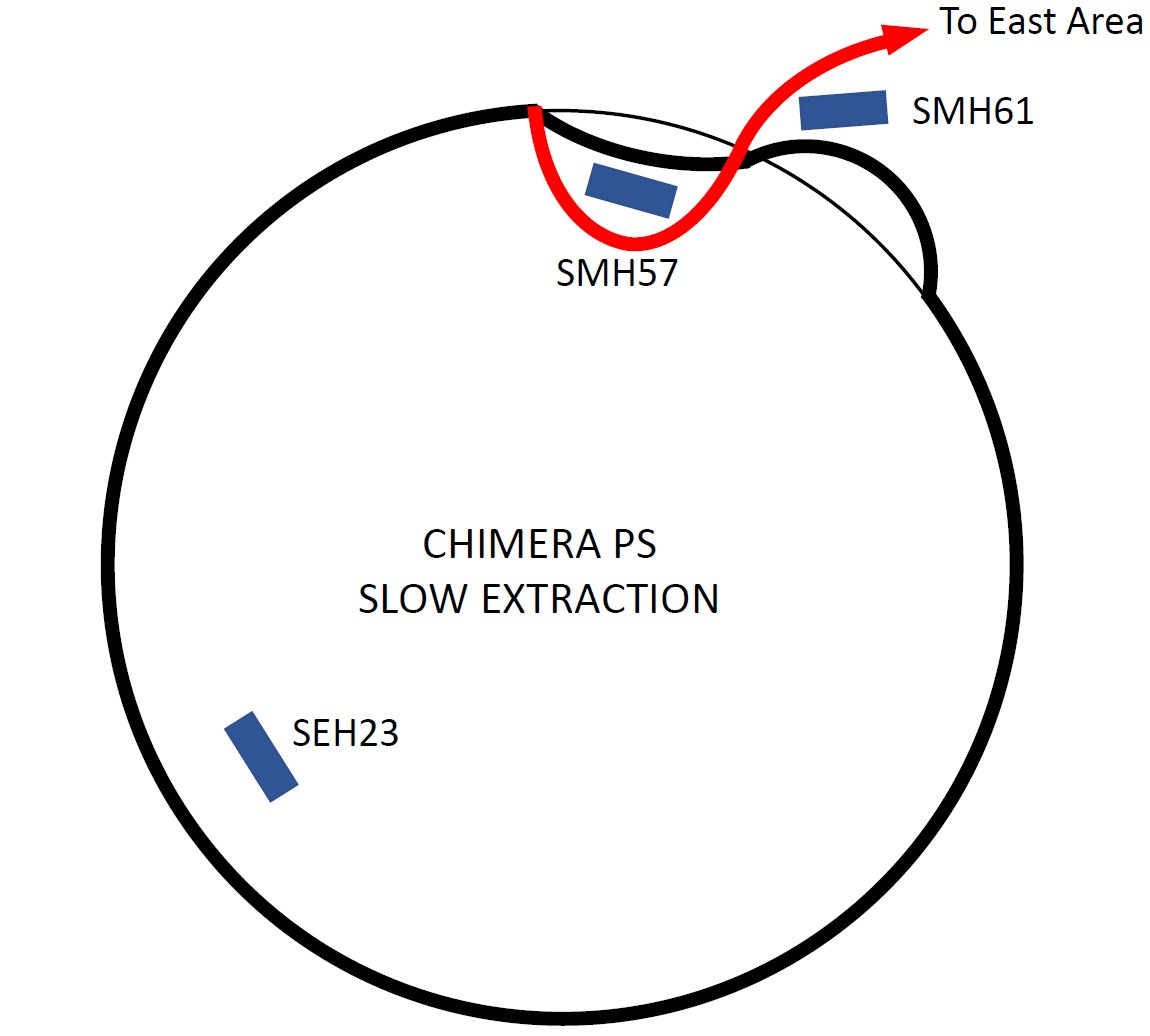
\includegraphics[width=0.4\textwidth]{images/SX_CHIMERA.jpg}
\caption{Slow extraction scheme for CHIMERA}
\label{fig:sx}
\end{figure}

The amplitude growth needed to jump the septum is done with slow extraction. Iteration on the scheme have been made, starting with a ramp on the low energy quadrupoles LEQ to increase to tune to the third integer resonant tune and converging on Radiofrequency knock out (RFKO) for a better control of the beam intensity at different energies (see section \ref{beam_intensity}).

For RFKO, the setup was to bring the tune of the beam close to the resonance (with the radial loop GRPOS as increase the tune with the LEQ would also change the tune but change the optics) and back off slightly in tune so that the Transverse Feedback Blowup (TFB) is used to push particles into resonance. Once we are close to the tune we turn of the radial loop and debunch the beam. The machine is static (nothing ramping). We chirp using the Q-meter. A low frequency, the chirps is visible in the spill but for faster chirping at 1ms the frequency is the spill is suppressed by the transit time.